\documentclass[10pt]{beamer}
\input{FrontMatter/preamble.tex}
\usepackage[spanish]{babel}
%\usetheme{Berlin}
\usetheme{CambridgeUS}

%\usecolortheme{senac}
\usecolortheme{seahorse}
\newcommand{\celda}[1]{
\begin{minipage}{2.5cm}
\vspace{5mm}
#1
\vspace{5mm}
\end{minipage}
}

\author[Jhon]{Jhon Gesell Villanueva Portella\inst{1}}
\title[Sesión 06]{Programación Orientada a Objetos}
\date{02 de octubre de 2020} 
\subtitle{Introducción a POO}
\logo{\includegraphics[scale=0.15]{makerlab.png}}
\institute[TLS]{
\inst{1}
Tolouse Lautrec.\\
\vspace{2mm}

}
\AtBeginSection[]
{
\begin{frame}<beamer>{Contenido}
\tableofcontents[currentsection,currentsubsection]
\end{frame}
}


\begin{document}
\begin{frame}
\maketitle
\end{frame}
\begin{frame}{Contenido}
\tableofcontents
\end{frame}
\section{Introducción}
\begin{frame}{Introducción}
\justifying
La Programación Orientada a Objetos (POO) es un paradigma fundamental en la programación para el desarrollo de cualquier software. A la fecha son la mayoría de lenguajes de alto nivel los que llegan a soportar la POO. como son Java, C\#, C++, Python, etc.

Por esta razón hablaremos de esta forma de pensar, de este paradigma que es la POO.

{\tiny Python Manizales - Jesse Padilla Agudelo}
\end{frame}

\begin{frame}{Introducción}
\justifying

\begin{figure}[H]
\centering
\includegraphics[scale=0.25]{Section_Files/images/01.png}
\caption{Imagen popular que asocia al lenguaje Python.}
\end{figure}

{\tiny Python Manizales - Jesse Padilla Agudelo}
\end{frame}

\begin{frame}{Programación Orientada a Objetos}
\justifying
La programación orientada a objetos es un paradigma de programación que busca representar entidades u objetos agrupando datos y métodos que puedan describir sus características y comportamientos.

{\tiny Python Manizales - Jesse Padilla Agudelo}
\end{frame}

\begin{frame}{Programación Orientada a Objetos}
\justifying
La POO paradigma de programación en el que los conceptos del mundo real relevantes para nuestro problema se modelan a través de clases y objetos, y en el que nuestro programa consiste en una serie de iteracciones entre estos objetos.

{\tiny Python Manizales - Jesse Padilla Agudelo}
\end{frame}

\begin{frame}{Ventajas de la POO}
\justifying
\begin{itemize}
\item Fomenta la reutilización y extensión del código.
\item Permite crear sistemas más complejos.
\item Relacionar el sistema al mundo real.
\item Facilita la creación de programas visuales.
\item Construcción de prototipos.
\item Agiliza el desarrollo de software.
\item Facilita el trabajo en equipo.
\item Facilita el mantenimiento de software.
\end{itemize}

{\tiny Python Manizales - Jesse Padilla Agudelo}
\end{frame}

\begin{frame}{Modelo Orientado a Objetos}
\justifying
\begin{itemize}
\item Objeto.
\item Clase.
\item Mensaje.
\item Método.
\item Interfaz
\item Herencia.
\end{itemize}

{\tiny Python Manizales - Jesse Padilla Agudelo}
\end{frame}
\section{Gestores de paquetes}
\begin{frame}{POO: El Objeto}
\justifying
\begin{itemize}
\item Un objeto es una unidad que engloba en sí mismo características y comportamiento necesario para procesar infomración. Cada objeto contiene datos y funciones. Y un programa se construye como un objeto de objetos, o como un único objeto.
\end{itemize}
{\tiny Python Manizales - Jesse Padilla Agudelo}
\end{frame}

\begin{frame}{POO: El Objeto}
\justifying
Ejemplo:
\begin{itemize}
\item Carro BMW.\\
Características:
	\begin{itemize}
	\item 4 ruedas 	Michelline.
	\item Motor BMW.
	\item Caja de cambios de 7 velocidades.
	\item Color Azul.
	\item 2 espejos.
	\end{itemize}
\end{itemize}
{\tiny Python Manizales - Jesse Padilla Agudelo}
\end{frame}

\begin{frame}{POO: La Clase}
\justifying
La clase es un modelo o prototipo que define las variables y métodos comunes a todos los objetos de cierta clase. También se puede decir que una clase es una plantilla genérica para un conjunto de objetos de similares características.

{\tiny Python Manizales - Jesse Padilla Agudelo}
\end{frame}

\begin{frame}{POO: La Clase}
\justifying

Ejemplo:
\begin{itemize}
\item Carro Vehículo.
	\begin{itemize}
	\item Número de ruedas.
	\item Tipo de Motor.
	\item Capacidad del tanque de gasolina.
	\item Número de velocidades de la caja de cambios.
	\item Color.
	\end{itemize}
\end{itemize}

{\tiny Python Manizales - Jesse Padilla Agudelo}
\end{frame}

\begin{frame}{POO: El Mensaje}
\justifying
\begin{itemize}
\item El mensaje es el modo en que se comunican los objetos entre si.\\
Ejemplo:
\begin{itemize}
\item Cuando llamemos a una función de un objeto, diremos que estamos enviando un mensaje a ese objeto.
\end{itemize}
\end{itemize}
{\tiny Python Manizales - Jesse Padilla Agudelo}
\end{frame}

\begin{frame}{POO: El Objeto}
\justifying
\begin{figure}[H]
\centering
\includegraphics[scale=0.35]{Section_Files/images/02.png}
\caption{Interfaz del Anaconda Navigator.}
\end{figure}
{\tiny Python Manizales - Jesse Padilla Agudelo}
\end{frame}


\section{Programación Orientada a Objetos}
\begin{frame}{Introducción a la Programación Orientada a Objetos}
\justifying
Para entender mejor la programación orientada a objetos, haremos un breve estudio sobre las causas fundamentales que llevaron a cabo la creación de la misma. Podemos resumir como causas principales las siguientes:

\begin{itemize}
\item La complejidad inherente al software.
\item La crisis del software.
\item Los Factores de la calidad del software.
\end{itemize}


{\tiny Fundamentos de Programación Orientada a Objetos por Ing. Isis Espinosa Salazar, página 13}
\end{frame}
%\section{Ejercicios}
%\begin{frame}{Polimorfismos}
\justifying


\end{frame}

%\section{Final}
%\begin{frame}{Eventos y Acciones}
\justifying

\end{frame}
		

%********************


\appendix
\section{Referencias}
%\subsection<presentation>*{Referencias}
\begin{frame}{Referencias}
\begin{thebibliography}{8}

\beamertemplatebookbibitems
% imagen de revista, paper o artículo
\bibitem{Author01}
Introducción a la Programación con Python
\newblock{\em Nilo Ney Coutinho Menezes}.
\newblock{Editorial Novatec (2016)}

\end{thebibliography}
\end{frame}

\end{document}

































